\documentclass[letterpaper,12pt]{article}
\usepackage[utf8]{inputenc}
\usepackage{graphicx}
\usepackage{amssymb,amsmath}
\usepackage{verbatim}
\usepackage[parfill]{parskip}
\usepackage{hyperref}
\usepackage{listings}

\title{Information Retrieval CS 834 : Assignment 3}
\author{Miranda Smith\\ msmit213@odu.edu}
\begin{document}
\maketitle
\date{}

\begin{abstract}
Exercise questions 6.1, 6.2, 6.4, 6.5, 6.9, 7.7, and MLN1 completed. Spring 2017. 
\end{abstract}

\pagebreak

\section{Problem 6.1}
 Using the Wikipedia collection provided at the book website, create a sample of stem clusters by the following process:
\begin{enumerate}
  \item Index the collection without stemming.
  \item Identify the first 1,000 words (in alphabetical order) in the index.
  \item Create stem classes by stemming these 1,000 words and recording which words become the same stem.
  \item Compute association measures (Dice’s coefficient) between all pairs of stems in each stem class. Compute co-occurrence at the document level.
  \item Create stem clusters by thresholding the association measure. All terms that are still connected to each other form the clusters.
\end{enumerate}
Compare the stem clusters to the stem classes in terms of size and the quality (in your opinion) of the groupings.

\subsection{Solution}

I completed this assignment using the Galago indexing functionality and my own python scripts.

\subsubsection{Indexing}

I installed Galago and used the ``galago build" command to create my index. Then I used the command ``galago dump-index" to get a csv file that I could process later.

\subsubsection{First 1000 Words}

To grab the first 1000 words of the index I created a python script, shown below, to open the csv file containing my index. I read the word for each line making sure it started with an alphabetic character, because the beginning of the file is made up of numbers that would be useless for stemming. I also had to make sure I wasn't grabbing any repeats because the csv has a row for a word every time it shows up in a different file.

\begin{lstlisting}[breaklines]

---------------------------------------------------------------
import csv

with open("indexedWords.csv", newline='') as csvfile, open("1000unstemmed.txt", "w") as outfile:
    freader = csv.reader(csvfile, delimiter=',')
    count = 0
    wordList = []
    for row in freader:
        if count > 1000:
            break
        if row[0].isalpha():
            if row[0] not in wordList:
                wordList.append(row[0])
                outfile.write(row[0])
                outfile.write("\n")
                count = count +1
---------------------------------------------------------------
\end{lstlisting}

\subsubsection{Create Stem Classes}

I created another python script, shown below, to take the output from the previous program and create stem classes. This program read in every word from the 1000 unique words and stemmed them with the Porter 2 stemmer. Then it creates another file to output the stem classes by printing out the base stem followed by the words that turn into that stem. An example of that file is shown below. Aggregating the words into stem classes left me with 109 classes.

\begin{lstlisting}[breaklines]
----------------------------------------------------------
from stemming.porter2 import stem
from collections import defaultdict

stemclass = defaultdict(list)
with open("1000unstemmed.txt", "r") as infile:
    words = infile.read().splitlines()
    for word in words:
        originalW = word
        stemW = stem(originalW)
        if len(stemW) > 0:
            stemclass[stemW].append(originalW)
classes = dict(stemclass)

with open("stemclass.txt", "w") as outfile:
    for key, value in sorted(classes.items()):
        if len(value) > 1:
            outfile.write(key + " ")
            for word in value:
                outfile.write(word + " ")
            outfile.write("\n")
----------------------------------------------------------
\end{lstlisting}


\begin{lstlisting}[breaklines]
                  Stem Classes
----------------------------------------------------------
\abad abad abadal 
\abandon abandon abandoned abandoning abandonment 
\abaqa abaqa abaqas 
\abb abb abbe abbs 
\abba abba abbas 
\abbasid abbasid abbasids 
\abbess abbess abbesses 
\abbey abbey abbeys 
\abbi abbi abbie abby abbys 
\abbot abbot abbots 
\abbott abbott abbotts 
\abbrevi abbreviated abbreviation abbreviations 
----------------------------------------------------------
\end{lstlisting}

\subsubsection{Create Stem Clusters with Dice's Coefficient}

In the program below, I created stem clusters by comparing each word in a stem class to the other words in the class with a term association measure. If the score between two words was above a certain threshold, which I empirically set to 0.05 because of the small size of the classes, then both of those words were kept for the stem cluster.

\begin{lstlisting}[breaklines]

----------------------------------------------------------
idx = defaultdict(list)
with open("indexedWords.csv", newline='') as csvfile, 
open("stemclass.txt", "r") as stemclass,
 open("stemcluster.txt", "w") as clusterFile:
    stemcluster = defaultdict(list)

    #read in the index
    freader = csv.reader(csvfile, delimiter=',')
    for row in freader:
        if row[0][0] == 'a':
            idx[row[0]].append(row[1])
        if row[0][0] == 'b':
            break
    index = dict(idx)
    #read in the stem classes
    for row in stemclass.read().splitlines():
        classStem = row.split()[0]
        classWords = row.split()[1:]
        #compare all pairs of words in a class
        for inx, wordA in enumerate(classWords):
            if inx != len(classWords)-1:
                for wordB in classWords[inx+1:]:
                    #compute dices coefficient
                    score = diceCoeff(wordA, wordB, index)
                    #if the score is above the threshold add WordA and Word B to the cluster
                    #and stop looking at this word A
                    if score >= THRESHOLD:
                        stemcluster[classStem].append(wordA)
                        stemcluster[classStem].append(wordB)
                        break
    #write the new cluster file
    clusters = dict(stemcluster)
    for key, value in sorted(clusters.items()):
        clusterFile.write(key + " ")
        #get rid of duplicates
        words = set(value)
        for word in words:
            clusterFile.write(word + " ")
        clusterFile.write("\n")
----------------------------------------------------------
\end{lstlisting}

The term association metric used was Dice's Coefficient. 

$$Term Association = \frac{2*n_{ab}}{ n_a * n_b}  $$

$n_{ab}$ is the number of documents containing the words A and B. $ n_a$ is the number of documents containing the word A. $ n_b$ is the number of documents containing the word B. 
This is implemented in the python script below. From the index a count of all the documents containing A and a count of all the document containing B is retrieved. The number of documents containing A and B is retrieved from the intersection of the previous two sets.

\begin{lstlisting}[breaklines]
----------------------------------------------------------
def diceCoeff(wordA, wordB, index):
    docsWA = index[wordA]
    nDocsWA= len(docsWA)
    docsWB = index[wordB]
    nDocsWB= len(docsWB)

    docsWAB = set(docsWA).intersection(docsWB)
    nDocsWAB = len(docsWAB)

    score = (2 * nDocsWAB)/(nDocsWA * nDocsWB)
    return score
----------------------------------------------------------
\end{lstlisting}


An example of the stem clusters file is shown below. The output has been reduced to only 36 stem clusters from 109 stem classes.
\begin{lstlisting}[breaklines]

----------------------------------------------------------
\aberr aberrations aberration 
\abjad abjads abjad 
\abomin abomination abominations 
\abort abort abortion 
\abrahamsen abrahamsens abrahamsen 
\abridg abridgment abridged abridges abridgement abridging 
\abrog abrogated abrogation 
\absent absented absent 
----------------------------------------------------------
\end{lstlisting}


\subsection{Evaluation of Classes versus Clusters}

Stem clusters are much smaller than stem classes. For these 1000 words there were 109 stem classes and only 36 stem clusters.
There are a few examples of stem classes that are clearly related to each other and should stay grouped together, such as 
\begin{lstlisting}[breaklines]

----------------------------------------------------------
\absorb absorb absorbable absorbance absorbed absorbency absorbent absorber absorbing absorbs 
\accept accept acceptable acceptance accepted accepting accepts 
----------------------------------------------------------
\end{lstlisting}

that were not kept as a group at all in the stem clusters. However, it did to a good job of breaking up classes like the one below.

\begin{lstlisting}[breaklines]

----------------------------------------------------------
\account account accountability accountable accountancy accountant accountants accounted accounting 
----------------------------------------------------------
\end{lstlisting}
A class that contains words for responsibility and money transactions into the following cluster focused solely on money.
\begin{lstlisting}[breaklines]

----------------------------------------------------------
\account accountancy accountants accountant 
----------------------------------------------------------
\end{lstlisting}

\pagebreak

\section{Problem 6.2}

Create a simple spelling corrector based on the noisy channel model. Use a single-word language model, and an error model where all errors with the same edit distance have the same probability. Only consider edit distances of 1 or 2. Implement your own edit distance calculator (example code can easily be found on the Web).

\subsection{Solution}

The noisy channel model says that a user chooses a word w based on a particular probability described by the language model. The probability that they would then write word e  given that they were trying to write the word w describes the error model. The more complex methods of determining the value of w given e takes into account the frequency of w in the corpus and the query log. The simpler method implemented here assumes that all words within an edit distance of 1 or 2 of word e have the same probability of being the word w.

Working spelling corrector. This program finds the misspelt word and suggests replacement words that are an edit distance of 2 or less. The example in \ref{correctworld} is correcting the shorter word ``wrld" that was meant to be ``world". The algorithm returns many options for the correction, because many options for the word are within the edit distance of 2. Figure \ref{correct birmingham} is trying to suggest a replacement for the misspelt ``brimingham". This word returns much less options for corrections because only ``birmingham" is within the proper edit distance, meaning the algorithm will be more precise for longer words.

\begin{figure}[h]
\centering
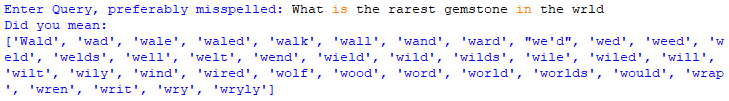
\includegraphics[scale=0.75]{data/62example1.png}
\caption{Correction suggestions for the word ``wrld"}
\label{correctworld}
\end{figure}

\begin{figure}[h]
\centering
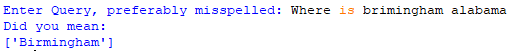
\includegraphics[scale=0.75]{data/62example2.png}
\caption{Correction suggestions for the word ``brimingham"}
\label{correct birmingham}
\end{figure}

The first step was to find the misspelt word in the query. I did this by comparing each word in the query to the dictionary in the department Unix systems that I copied to my own dictionary file, making sure to account for case. The function below implements this by taking a string and returning the first word it finds that is misspelt.

\begin{lstlisting}[breaklines]
----------------------------------------------------------
def findMissspelledWord(string):
        with open("dictwords.txt", "r") as dictFile:
                dictionary = dictFile.read().splitlines()
                upDict = [x.upper() for x in dictionary]
                for word in string.split(' '):
                        if word.upper() in upDict:
                                pass
                        else:
                                return word
        return ""
----------------------------------------------------------
\end{lstlisting}

Once I have the misspelt word I made an assumption that the first letter of the misspelt word would be correct and collected from the dictionary all of the words starting with the same letter. These words were then compared against the misspelt word to determine if the edit distance was within the correct tolerance to be considered a replacement word. The edit distance was calculated with the damerau levenshtein distance shown below. This algorithm was taken from an example online from Guy Rutenberg after determining that it would correctly list a transposition edit as a distance of 1 instead of 2, which many examples online do not. The damerau levenshtein distance says that a deletion, insertion, or substitution of a character in a word, along with the transposition of two characters is an edit distance of 1. The number of changes necessary to turn one word into another is the edit distance for those two words.

\begin{lstlisting}[breaklines]
----------------------------------------------------------
#levenshtein distance code from Guy Rutenberg
#https://www.guyrutenberg.com/2008/12/15/damerau-levenshtein-distance-in-python/
def damerau_levenshtein_distance(s1, s2):
    d = {}
    lenstr1 = len(s1)
    lenstr2 = len(s2)
    for i in range(-1,lenstr1+1):
        d[(i,-1)] = i+1
    for j in range(-1,lenstr2+1):
        d[(-1,j)] = j+1
    for i in range(lenstr1):
        for j in range(lenstr2):
            if s1[i] == s2[j]:
                cost = 0
            else:
                cost = 1
            d[(i,j)] = min(
                           d[(i-1,j)] + 1, # deletion
                           d[(i,j-1)] + 1, # insertion
                           d[(i-1,j-1)] + cost, # substitution
                          )
            if i and j and s1[i]==s2[j-1] and s1[i-1] == s2[j]:
                d[(i,j)] = min (d[(i,j)], d[i-2,j-2] + cost) # transposition
    return d[lenstr1-1,lenstr2-1]
----------------------------------------------------------
\end{lstlisting}

\pagebreak

\section{Problem 6.4}

Assuming you had a gazetteer of place names available, sketch out an algorithm for detecting place names or locations in queries. Show examples of the types of queries where your algorithm would succeed and where it would fail.

\section{Solution}

The simplest approach would be to run every query word through the gazetteer to find any location information. However, the brute force method would seriously hurt response time. One way to fix that is to narrow the size of the gazetteer based on the location of the user. If location data is known, such as mobile phone GPS data, then the gazetteer could be focused on regional information with a courser view on the rest of the world. For example, location information in different countries would be limited to major landmarks, major cities, and country names while information for the local region would have street names, stores, and neighboring city information. Most people do not travel and if they do, not frequently, so most user queries are focused on local information. Unless the user has a history of querying about a different location, then they are likely to know very little about geographical information for distant places and thus not likely to query it.

To save more time the query could be processed through a set of templates to discover the likelihood of location information being present before searching through the gazetteer. Some examples of those templates are shown below.

 \begin{lstlisting}[breaklines]
----------------------------------------------------------
directions to _
_ near me
weather in _
restaurants
location of _
ave| blvd | st| rd | bch | aly | brg | byp | ct | ....
movie times
flights to _
local _
...
----------------------------------------------------------
\end{lstlisting}

The best approach would be to incorporate relevance feedback if query history is available. Through the query history commonly searched areas can be found and matched against the query as the first step of location information identification, then the query could be run through the templates which could lead to searching through the rest of the gazetteer not commonly searched or local. The algorithm would do poorly at first without any query history, but would still operate well with the parsed down gazetteer described earlier. Once more query history is available the algorithm should improve. A few queries that would fail in this algorithm include ``dog parks" which the user would need to refine to ``dog parks near me" or "directions to a dog park". Another query that would fail is ``radiator for a Ford Explorer" assuming the user was trying to shop for one, this query would not realize it needed to find local auto parts stores.

\pagebreak

\section{Problem 6.5}

Describe the snippet generation algorithm in Galago. Would this algorithm work well for pages with little text content? Describe in detail how you would modify the algorithm to improve it.

\subsection{Solution}


Snippet generation in Galago is based off query term matching. It creates a snippet region, or sentence fragment, for every query term occurrence in the document. For each snippet it checks if it overlaps, and combines those regions. It then adds that snippet region to the final snippet until the final snippet would exceed a particular size restriction. If it would exceed the limit, the program checks the snippet regions after it to see if any could fit in it's place. This means that the final snippet will be as close as possible to the character limit, but would not go over it. It is also heavliy biased towards query words that occur sooner in the document.

The code for snippet generation is found in the Galago source code in the file SnippetGenerator.java.

This algorithm would work fine for pages with little text content. It would just show as much text as it could as long as it found a matching term in the document. The drawback comes when there are no exact word matches in the document body as shown in Figure \ref{nosnippet}. This shows that 3 out of the top 5 returned pages have no snippet generated. The document has already been determined to be relevant, so the query terms might be in the title, or there may be stemmed versions of the word inside the document that would not be chosen for the snippet. Another drawback is that more important and relevant information than  in the snippet may be further down in the document that wouldn't be included in the snippet because of it's location. A good example is Figure \ref{badsnippet}, this document has the answer to the query at the end of the first paragraph, but because unimportant query terms show up earlier those get priority. 

\begin{figure}[h]
\centering
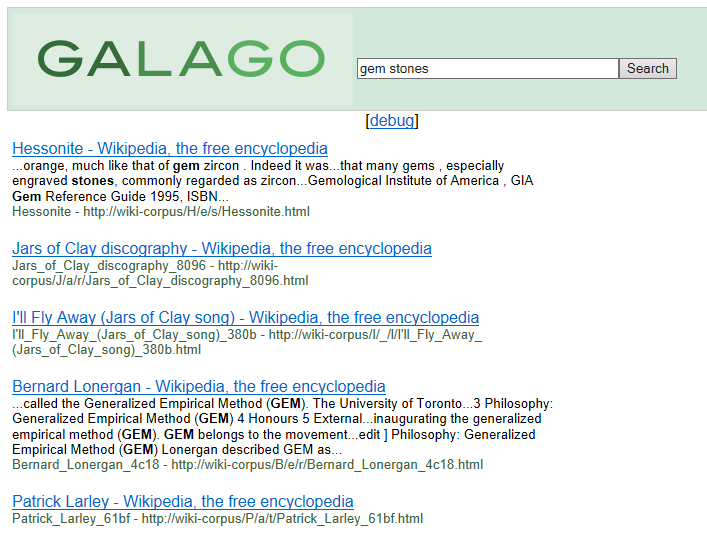
\includegraphics[scale=0.75]{data/65nosnippet.png}
\caption{No snippet generated for top rated documents}
\label{nosnippet}
\end{figure}

\begin{figure}[h]
\centering
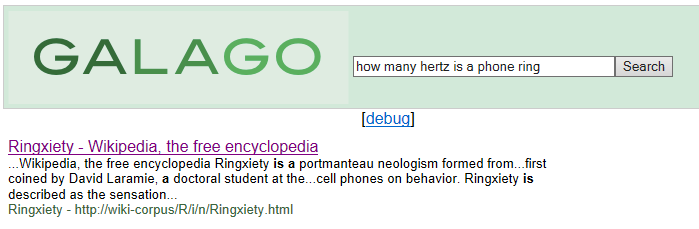
\includegraphics[scale=0.75]{data/65importantInfo.png}
\caption{Unimportant info in snippet}
\label{badsnippet}
\end{figure}

An improved implementation would involve scoring each snippet and adding the highest scoring snippets to the final snippet until the final snippet length is reached. It appears that a potential implementation for that has been created and included in the code. However, it is not being used in the current code flow and a comment indicates that it is too slow for practical use in snippet generation. One possible improvement is to include stemming logic to expand the amount of matches found in the document. If no matches are found at all it would still be better to show the first few sentences of the document than to show nothing when there are no matches.

\pagebreak


\section{Problem 6.9}

Give five examples of web page translation that you think is poor. Why do you think the translation failed?


\subsection{Solution}
I created English queries and with google translate, found the equivalent query in another language. That query was then entered into a google search with the language settings set to the same language as the query. I then selected a foreign language website and entered it's URI into Bing translate to see the English translated version of that page. This process helped me find websites that were not news and hopefully harder to translate. /ref{Example2} also includes a Facebook post that Facebook translated with it's in house translator.  

\subsubsection{Example 1}

This\href{https://kotobank.jp/word/\%E9\%89\%A2\%E6\%A4\%8D\%E3\%81\%88-601905}{website} is about a Japanese person's potted plant in commemoration of their husband. The text from the web page is shown below.

\begin{lstlisting}[breaklines]

----------------------------------------------------------
Nikko, Kinugawa hot springs waterfall Tomoko Shimada (78) in the House last month, potted cereus bloomed. Than usual this year put more than 30 rings of white flowers. It was painstakingly crafted Toshio's husband died suddenly at the age of 82 in February from 13 years ago and grew flowers.

Tomoko moved from Nagano Prefecture Omachi city Kinugawa in the fourth grade of elementary school. After the shamisen from elementary school, Geisha who has taught in the town. Toshio, worked at the long-established ryokan and married in 1963. Blessed with two children, has three grandchildren.

Toshio-San retired hotel manager finally. Retirement as city Commissioners listen to consult residents on the other hand, began growing in the garden of a home cereus from 13 years ago.

Cereus Cactus family in the evening.
----------------------------------------------------------
\end{lstlisting}

The first two paragraphs are confusing due to  having the words out of order but still has enough key words to be understandable. However the third paragraph has the words mix up enough to be unintelligible. The reason for this bad translation is probably a feature of the language itself. The original website is in Japanese and compared to English the parts of speech are structured very differently and is most likely the cause of the bad translation. The translation was done through \href{http://www.microsofttranslator.com/bv.aspx?to=en&r=true&a=http\%3A\%2F\%2Fwww.asahi.com\%2Farticles\%2FASK944SHKK94UUHB009.html\%3Fref\%3Dchiezou}{Bing}.

\subsubsection{Example 2}

Figure \ref{bad FB translation} is in Japanese and it is a Facebook post from one of my friends who is my old Japanese teacher.

\begin{figure}[h]
\centering
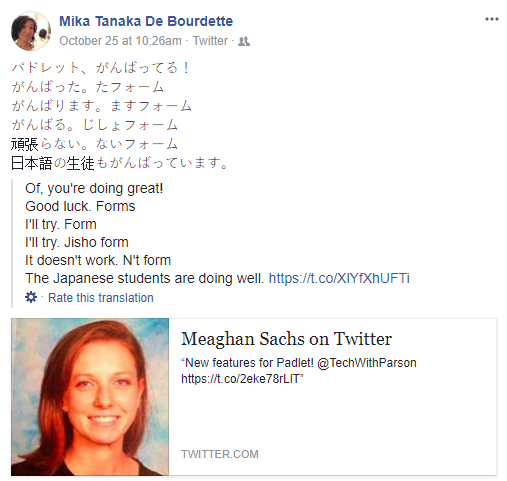
\includegraphics[scale=0.75]{data/FacebookExampleBadTranslation.png}
\caption{Translated Japanese Facebook post}
\label{bad FB translation}
\end{figure}

Beyond the encouraging nature of the post, most of the post makes not sense and has no meaning. Facebook uses their own translator and it probably suffers from the same issues Bing does with ordering, however this translation has done an even worse job of translating the key word that would make this understandable.

\subsubsection{Example 3}

This example is a web page about the weather in Urdu. I chose Urdu because I know it is a very infrequently used language and would be very difficult for translators. The original website is shown in Figure \ref{Urdu Original}. While a part of the translation through Bing is shown in Figure \ref{Urdu Bad}. The translator doesn't recognize the characters and instead is showing the actual code of the page because it no longer even knows how to parse it.

\begin{figure}[h]
\centering
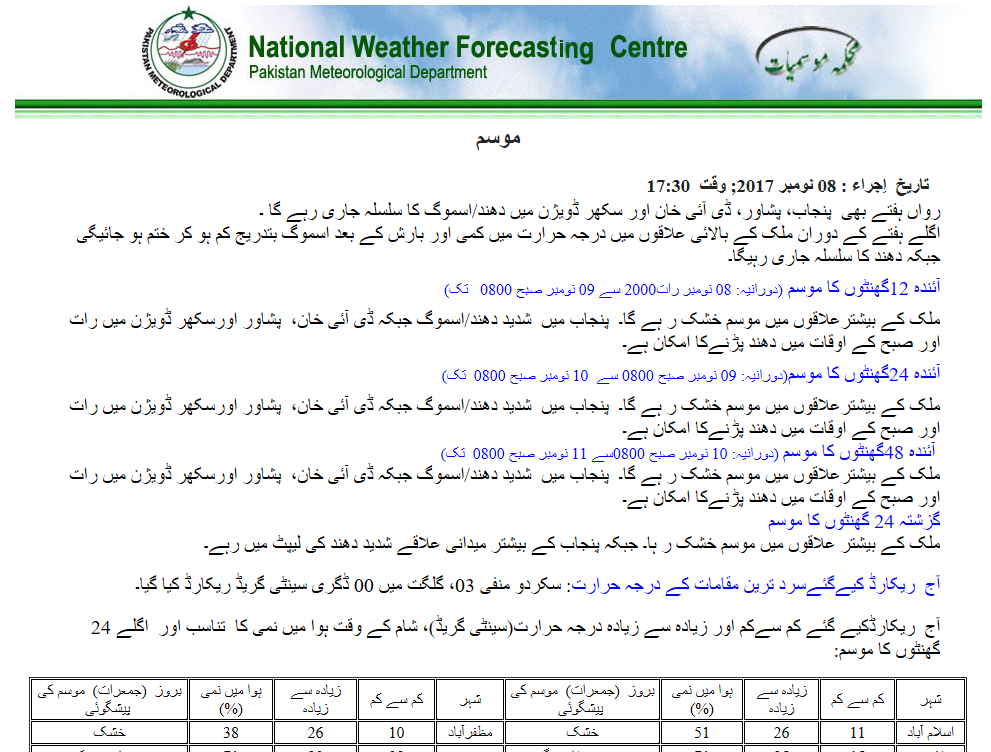
\includegraphics[scale=0.5]{data/69urduWeatherOrig.png}
\caption{A page about the weather in Urdu}
\label{Urdu Original}
\end{figure}

\begin{figure}[h]
\centering
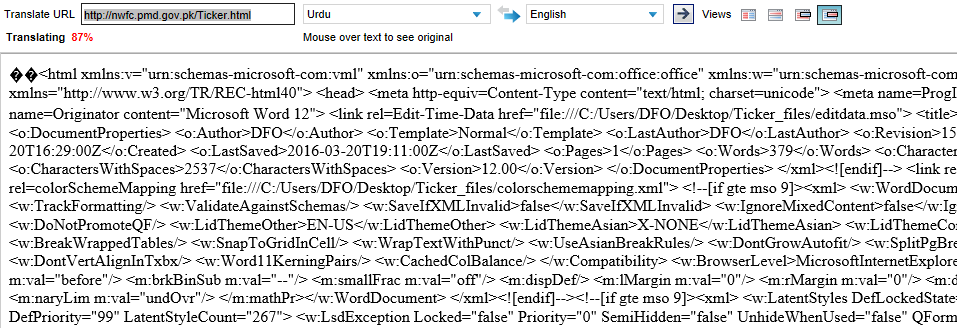
\includegraphics[scale=0.5]{data/69urduWeatherBad.png}
\caption{A badly translated page about the weather in Urdu}
\label{Urdu Bad}
\end{figure}

\subsubsection{Example 4}

This example shows a Chinese web page talking about how to chose a new school in Canada. The original page is shown in Figure \ref{chinese orig} while the translated page is in Figure \ref{chinese bad}. The translation itself is fairly good, however in the process of translation the web page format was destroyed. The header is now being shown over the text of the document and makes it hard to read.


\begin{figure}[h]
\centering

\includegraphics[scale=0.5]{data/SchoolExampleOrig.png}
\caption{A page in Chinese about choosing a good school}
\label{chinese orig}
\end{figure}

\begin{figure}[h]
\centering
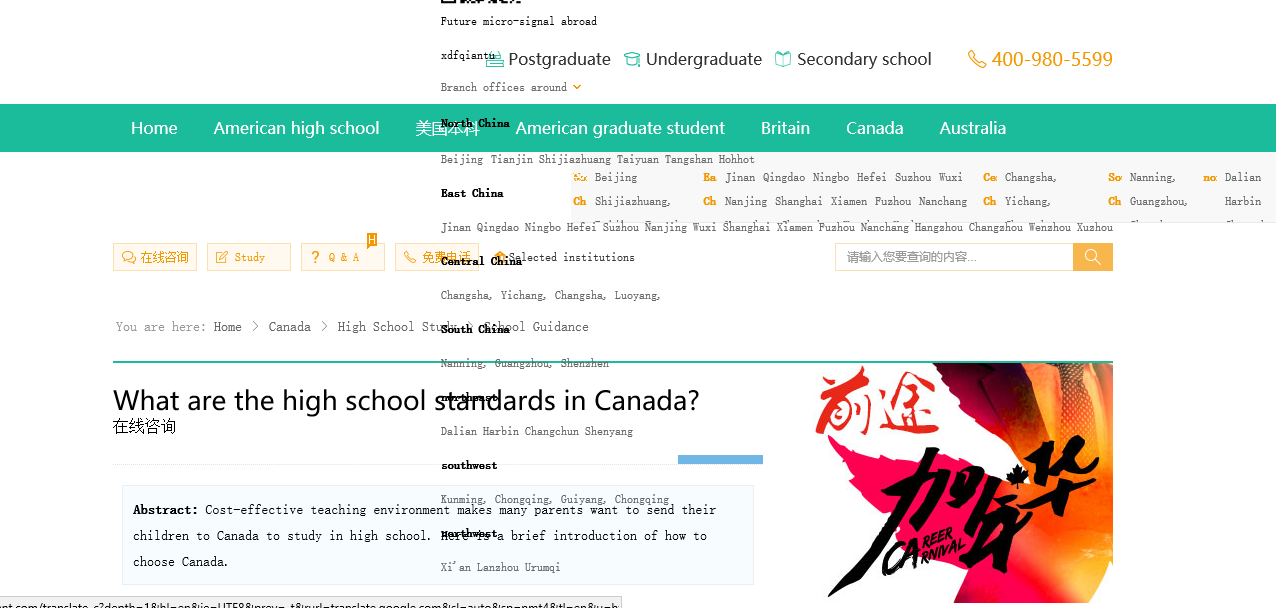
\includegraphics[scale=0.5]{data/SchoolExampleBadTranslation.png}
\caption{A translated page about chosing a good school}
\label{chinese bad}
\end{figure}

\subsubsection{Example 5}

The last example is of a  \href{http://www.hankookilbo.com/v/095b018d7b2344cb810f4c44de5779d7}{blog} in Korean. When translated through Bing it shows output like the following.


\begin{lstlisting}[breaklines]

----------------------------------------------------------
Hyundai Accent sedan `` entry in the ' change advanced options for some designs apply zoom ``caustic ' to change the model of a beached year my gun.
----------------------------------------------------------
\end{lstlisting}

This example shows a clear misinterpretation of some words like ``gun", ``beached" and ``caustic" which we can safely assume are not actually in the blog at all.

\pagebreak

\section{Problem 7.7}

What is the ``bucket” analogy for a bigram language model? Give examples.

\subsection{Solution}

The ``bucket" analogy for the uni-gram model is when we imagine the language model for that document as a bucket of words. The probability of choosing a word out of the bucket is determined by how many instances of the word is in the bucket or document. Using this bucket, or language model, we pick a word out of the bucket, write it down, and put it back into the bucket and drawing again. So the words are considered independent and the probability of choosing a particular word depends on its frequency.

For the bi-gram language model terms are now the combination of two words that appear next to each other in the document. So each word is going to appear in the bucket multiple times for each occurrence in the document combined with different words.

If the document is

\begin{lstlisting}[breaklines]

----------------------------------------------------------
Somebody poisoned the waterhole. There's a snake in my boot.
----------------------------------------------------------
\end{lstlisting}

The terms in the ``bucket", if we remove stop words like ``the" and ``and" will be:

\begin{lstlisting}[breaklines]
----------------------------------------------------------
Somebody poisoned 
poisoned waterhole 
waterhole There 
There snake
snake in 
in my 
my boot
----------------------------------------------------------
\end{lstlisting}

So now instead of being able to pick words one at a time from the bucket and ending up with a phrase like ``boot poisoned snake there waterhole" to describe the document we pick one term at a time, containing two words. An example output for this bi-gram model might be ``poisoned waterhole poisoned waterhole in my somebody poisoned waterhole there" which is still not likely to make syntactical sense but it provides some context to each word.

\pagebreak

\section{Problem MLN1}
Using the small Wikipedia example, choose 10 words and create stem classes as per the algorithm on pp. 191-192.

Algorithm on p 191:
\begin{enumerate}
  \item For all pairs of words in the stem classes, count how often they co-occur in text windows of W words.W is typically in the range 50–100.
  \item Compute a co-occurrence or association metric for each pair. This measures how strong the association is between the words.
  \item Construct a graph where the vertices represent words and the edges are between words whose co-occurrence metric is above a threshold T.
  \item Find the connected components of this graph. These are the new stem classes.
\end{enumerate}


\subsection{Solution}

I chose 10 words that were likely to form multiple clusters based off the classes and clusters in section \ref{Problem 6.1}. I also chose a few that were broken up when transforming the classes into clusters.

To create the stem classes I repeated the process in Section \ref{Create Stem Classes}.

To create the clusters I computed the Dice's Coefficient for each pair of terms in a class, except instead of doing the co-occurrence by document I did it by a window size. The modified section of code is below.

\begin{lstlisting}[breaklines]
----------------------------------------------------------
WINDOWSIZE = 75
def diceCoeff(wordA, wordB, index):
    docsWA = index[wordA]
    nDocsWA= len(docsWA)
    docsWB = index[wordB]
    nDocsWB= len(docsWB)
        
    docsWAB = set(docsWA).intersection(docsWB)
    nWinWAB =0
    #In Window
    for doc in docsWAB:
        for Aposition in docsWA[doc]:
            for Bposition in docsWB[doc]:
                if abs(int(Bposition)- int(Aposition)) <= WINDOWSIZE:
                    nWinWAB = nWinWAB + 1
    

    score = (2 * nWinWAB)/(nDocsWA * nDocsWB)
    return score
----------------------------------------------------------
\end{lstlisting}

I modified the index to be a three level dictionary, so that it could also store the position the words occurred in the document. I compared the positions of word A and B when they were found to be in the same document and checked if the distance was within the window. 

The resulting clusters are listed below. This evaluation made it so the 10 words, reduced to 3 classes, were further reduced to 2 clusters shown below.

 \begin{lstlisting}[breaklines]
----------------------------------------------------------
\abridg abridges abridged 
\acceler accelerate accelerates 
----------------------------------------------------------
\end{lstlisting}

It seems that the clusters seem to reduce the stem classes too far. One example is that ``accelerated" has been removed from the cluster, when syntactically it belongs in that cluster. I don't believe that two words appearing the in same window means that they are related or not. Most writers wouldn't be repeating themselves often enough and with different versions of words they've already typed in a close enough window for this algorithm to benefit.

\pagebreak

\end{document}